\documentclass[10pt,a4paper]{article}
\usepackage[utf8]{inputenc}
\usepackage[a4paper, margin=1.8cm, top=2.0cm, bottom=2.0cm]{geometry}
\usepackage{amsmath,amssymb}
\usepackage{xcolor}
\usepackage[most]{tcolorbox}
\usepackage{booktabs}
\usepackage{colortbl}
\usepackage{fancyhdr}
\usepackage{graphicx}
\usepackage{enumitem}

% Exact colors from original summary
\definecolor{themeblue}{rgb}{0.1686, 0.3529, 0.5294}   % #2B5A87
\definecolor{lightbg}{rgb}{0.9098, 0.9333, 0.9569}     % #E8EEF4
\definecolor{accentred}{rgb}{0.7843, 0.2706, 0.2275}   % #C8453A

% Header and Footer
\pagestyle{fancy}
\fancyhf{}
\fancyhead[L]{\textcolor{themeblue}{\small Lecture 2 --- Data exploration}}
\fancyhead[R]{\textcolor{themeblue}{\small Summary Sheet}}
\renewcommand{\headrulewidth}{0.5pt}
\renewcommand{\headrule}{\hbox to\headwidth{\color{themeblue}\leaders\hrule height \headrulewidth\hfill}}
\fancyfoot[C]{\thepage}

\begin{document}

% Title Block
\begin{center}
    {\LARGE\bfseries\color{themeblue} PCA}\\[3pt]
    {\small\itshape Summary sheet --- Deep Learning (S.-A. Berrani, ENSIA 2026--2027)}\\[3pt]
    \textcolor{themeblue}{\rule{\textwidth}{0.6pt}}
\end{center}

% Core Idea Box (Bulky notation bullets removed as requested)
\begin{tcolorbox}[
    colframe=themeblue,
    colback=lightbg,
    coltitle=white,
    fonttitle=\bfseries\sffamily,
    title={Core idea \& notation},
    arc=2mm,
    boxrule=0.6pt,
    left=8pt, right=8pt, top=6pt, bottom=6pt
]
\textbf{PCA} is a purely \textit{descriptive}, exploratory method (no probabilistic model assumed, normality not required) that handles any number of quantitative variables. It moves from $p$ variables to $q < p$ new variables while distorting reality as little as possible.
\end{tcolorbox}

\vspace{4pt}

% Section 1
\noindent{\Large\bfseries\color{themeblue} 1. Goal and principle}\\[4pt]
\textbf{Goal:} find the projection that \textbf{minimizes information loss}, i.e. the one that \textbf{maximizes the dispersion} of the projected data.\\
\textbf{Variance (dispersion):} mean squared distance between the points and their centroid $c$:
\[
V = \frac{1}{n} \sum_{i=1}^n d^2(x_i, c)
\]
\textbf{Property:} going from $p$ to $q < p$ necessarily loses dispersion. The idea is to lose as little as possible by choosing the projection axes well.\\[4pt]
\begin{tcolorbox}[
    colframe=accentred,
    colback=white,
    arc=1.5mm,
    boxrule=0.5pt,
    left=8pt, right=8pt, top=5pt, bottom=5pt
]
\textbf{Key principle of PCA.} Choose the projection (the axes) so as to \textit{maximize the dispersion} of the projected points.
\end{tcolorbox}

\vspace{6pt}

% Section 2 (Old Section 2 removed, Old Section 3 Algorithm expanded with how-to formulas)
\noindent{\Large\bfseries\color{themeblue} 2. Algorithm}\\[4pt]
Given a data matrix $X$ of size $n \times p$ ($n$ individuals, $p$ quantitative variables):

\begin{enumerate}[leftmargin=18pt, itemsep=4pt, topsep=2pt]
    \item \textbf{Center (and scale) data $X$ (Normalization):}
    \begin{itemize}[leftmargin=12pt, itemsep=2pt]
        \item Compute column means: $\bar{x}_k = \frac{1}{n}\sum_{i=1}^n x_{ik}$.
        \item Center: $x_{ik} \leftarrow x_{ik} - \bar{x}_k$.
        \item If variables have different units/scales, divide by standard deviation: $x_{ik} \leftarrow \frac{x_{ik} - \bar{x}_k}{\sigma_k}$.
    \end{itemize}

    \item \textbf{Calculate the covariance matrix:}
    \[
    C = X^T X \quad (p \times p)
    \]

    \item \textbf{Compute eigenvalues and eigenvectors of $X^T X$:}
    \begin{itemize}[leftmargin=12pt, itemsep=3pt]
        \item \textbf{Eigenvalues ($a_i$):} Solve the characteristic equation:
        \[
        \det(X^T X - a I) = 0
        \]
        \item \textbf{Eigenvectors ($v_i$):} For each eigenvalue $a_i$, solve the linear system:
        \[
        (X^T X - a_i I) v_i = 0 \quad \text{such that} \quad \|v_i\| = 1 \quad \left(\sum_{k=1}^p (v_{ik})^2 = 1\right)
        \]
    \end{itemize}

    \item \textbf{Order the pairs $(a_i, v_i)$ in descending order of eigenvalues:}
    \[
    a_1 \ge a_2 \ge \dots \ge a_p \ge 0
    \]
    Here, the eigenvalue $a_i$ equals the inertia (variance) carried by the principal axis $v_i$.

    \item \textbf{Keep the first $q$ pairs to construct the projection matrix $V$:}
    \[
    V = \begin{bmatrix} v_1 & v_2 & \dots & v_q \end{bmatrix} \quad (p \times q)
    \]

    \item \textbf{Project the individuals into the new space:}
    \[
    U = X V \quad (n \times q) \qquad \text{entry by entry: } u_i^j = \langle x_i, v_j \rangle = \sum_{k=1}^p x_{ik} v_{jk}
    \]
\end{enumerate}

\vspace{3pt}
\begin{center}
\small
\begin{tabular}{lll}
\toprule
\rowcolor{lightbg}
 & \textbf{Centering only} & \textbf{Centering + scaling} \\
\midrule
\textbf{Operation} & subtract the mean of each variable & also divide by the standard deviation \\
\addlinespace[3pt]
\textbf{Use when} & variables are \textit{homogeneous} (same unit, scale) & variables are \textit{heterogeneous} \\
\bottomrule
\end{tabular}
\end{center}

\vspace{3pt}
\begin{tcolorbox}[
    colframe=accentred,
    colback=white,
    arc=1.5mm,
    boxrule=0.5pt,
    left=8pt, right=8pt, top=4pt, bottom=4pt
]
\textbf{\color{accentred}Outliers.} PCA is very sensitive to noise: a few outliers can artificially rotate principal axes and alter the number of components needed to reach the target explained variance.
\end{tcolorbox}

% newpage

% Section 3 (Old Section 4)
\noindent{\Large\bfseries\color{themeblue} 3. Worked example with $X, U, V$ (toy data, $n=4, p=2$)}\\[4pt]
\textbf{Setup:} four individuals, two variables, columns already centered (sums = 0) and of the same scale:
\[
X = \begin{pmatrix} 2 & 1 \\ 1 & 2 \\ -1 & -2 \\ -2 & -1 \end{pmatrix} \quad (4 \times 2)
\]
\begin{enumerate}[leftmargin=18pt, itemsep=3pt, topsep=2pt]
    \item \textbf{Center/reduce:} column means are $0 \Rightarrow$ nothing to subtract; same scale $\Rightarrow$ no scaling.
    \item \textbf{Covariance matrix:} $X^T X = \begin{pmatrix} 10 & 8 \\ 8 & 10 \end{pmatrix}$.
    \item \textbf{Eigen-decomposition:}
    \[
    \det(X^T X - a I) = (10 - a)^2 - 64 = 0 \implies a_1 = 18, \quad a_2 = 2
    \]
    Eigenvectors: $(X^TX - 18I)v_1 = 0 \implies v_1 = \frac{1}{\sqrt{2}}\begin{pmatrix} 1 \\ 1 \end{pmatrix}$; \quad
    $(X^TX - 2I)v_2 = 0 \implies v_2 = \frac{1}{\sqrt{2}}\begin{pmatrix} 1 \\ -1 \end{pmatrix}$.
    \item \textbf{Sort:} $(a_1, v_1) = \left(18, \frac{1}{\sqrt{2}}\begin{pmatrix}1\\1\end{pmatrix}\right)$, then $(a_2, v_2) = \left(2, \frac{1}{\sqrt{2}}\begin{pmatrix}1\\-1\end{pmatrix}\right)$.
    \item \textbf{Keep $q = 1$:} $V = v_1 = \frac{1}{\sqrt{2}}\begin{pmatrix} 1 \\ 1 \end{pmatrix}$ ($p \times q = 2 \times 1$).
    \item \textbf{Project:} $U = XV$ ($4 \times 1$); with all axes kept, $V = [v_1 \ v_2]$ and $U$ is $4 \times 2$:
    \[
    U = XV = \frac{1}{\sqrt{2}}\begin{pmatrix} 3 & 1 \\ 3 & -1 \\ -3 & 1 \\ -3 & -1 \end{pmatrix}, \qquad \text{e.g. } u_1^1 = \frac{2\cdot 1 + 1\cdot 1}{\sqrt{2}} = \frac{3}{\sqrt{2}} \approx 2.12
    \]
\end{enumerate}
\textbf{Result:} the first column of $U$ ($= u^1$) is the $q = 1$ representation. Reconstruction with $q = 1$: $X' = u^1 v_1^T$ gives row 1 $= (1.5, 1.5)$ instead of $(2, 1)$; error $J = \|X - X'\|_F^2 = 4 \times 0.5 = 2 = a_2$ (the discarded eigenvalue). Explained variance: $\frac{18}{18+2} = \mathbf{90\%}$.

\vspace{8pt}

% Section 4 (Old Section 5)
\noindent{\Large\bfseries\color{themeblue} 4. Explained variance: choosing $q$}\\[4pt]
Choose the smallest $q$ such that the cumulative explained variance meets a chosen threshold $s$:
\[
\frac{\sum_{i=1}^q a_i}{\sum_{i=1}^p a_i} \ge s
\]
Since $a_i$ is the inertia of axis $i$, this represents the proportion of total information retained.
\begin{center}
\small
\begin{tabular}{lcccc}
\toprule
\rowcolor{lightbg}
\textbf{Axis} & 1 & 2 & 3 & 4 \\
\midrule
Eigenvalue $a_i$ (lecture, 4 grades) & 28.23 & 12.03 & 0.03 & 0.01 \\
Explained variance & 0.70 & 0.30 & 0.00 & 0.00 \\
Cumulative & 0.70 & 1.00 & 1.00 & 1.00 \\
\midrule
Toy example above & 18 & 2 & --- & --- \\
Explained / cumulative & 0.90 & 0.10 / 1.00 & --- & --- \\
\bottomrule
\end{tabular}
\end{center}
\vspace{-2pt}
\noindent In the lecture's grades example ($\sum a_i = 40.30$), $q = 2$ retains $\approx 100\%$ of the total information.

% newpage

% Section 5 (Old Section 6)
\noindent{\Large\bfseries\color{themeblue} 5. Studying the variables: flip the table and use correlations}\\[4pt]
\textbf{Idea:} position yourself in a different space by transposing the data perspective. Each initial variable $X^i$ (column $i$ of $X$) and each principal component $c^j$ (column $j$ of $U$) is viewed as a vector in $\mathbb{R}^n$.\\[4pt]
\textbf{Goal:} analyze the linear correlation coefficients $r(c^j, X^i)$ between initial variables and principal components.

\begin{enumerate}[leftmargin=18pt, itemsep=3pt, topsep=2pt]
    \item \textbf{Compute principal components:} $U = XV$ (columns $c^j = u^j$).
    \item \textbf{Compute correlation for every variable $i$ and axis $j$:}
    \[
    r(c^j, X^i) = \frac{\sum_k u_k^j x_k^i}{\sqrt{\sum_k (u_k^j)^2}\sqrt{\sum_k (x_k^i)^2}} \qquad \text{(since columns are centered)}
    \]
    \item \textbf{Gather in a $p \times q$ table of correlations} (``variables-factors'').
    \item \textbf{Plot variable $X^i$ as point $\big(r(c^1, X^i), r(c^2, X^i)\big)$ inside the correlation circle.}
    \item \textbf{Interpretation:} arrows close to each other $\Rightarrow$ strong positive correlation ($\approx 1$); orthogonal arrows $\Rightarrow$ uncorrelated ($\approx 0$); opposite arrows $\Rightarrow$ negative correlation ($\approx -1$).
\end{enumerate}

\noindent\textcolor{accentred}{\textbf{Example (toy data):}} $x^1 = (2, 1, -1, -2)$, $x^2 = (1, 2, -2, -1)$, $u^1 = \frac{1}{\sqrt{2}}(3, 3, -3, -3)$, $u^2 = \frac{1}{\sqrt{2}}(1, -1, 1, -1)$:
\[
r(c^1, X^1) = \frac{18/\sqrt{2}}{\sqrt{18}\sqrt{10}} = \frac{3}{\sqrt{10}} \approx 0.95, \qquad r(c^2, X^1) = \frac{\sqrt{2}}{\sqrt{2}\sqrt{10}} = \frac{1}{\sqrt{10}} \approx 0.32
\]

\begin{center}
\small
\begin{tabular}{lcc}
\toprule
\rowcolor{lightbg}
\textbf{Variable} & $c^1$ (90\%) & $c^2$ (10\%) \\
\midrule
$X^1$ & 0.95 & 0.32 \\
$X^2$ & 0.95 & $-0.32$ \\
\bottomrule
\end{tabular}
\end{center}
\vspace{-2pt}
\noindent\textit{Shortcut:} since $X^T u^j = a_j v_j$, $r(c^j, X^i) = v_j^i \frac{\sqrt{a_j}}{\|x^i\|}$. Check: $0.95^2 + 0.32^2 = 1$ (length = 1 on the circle).

\vspace{6pt}
\begin{center}
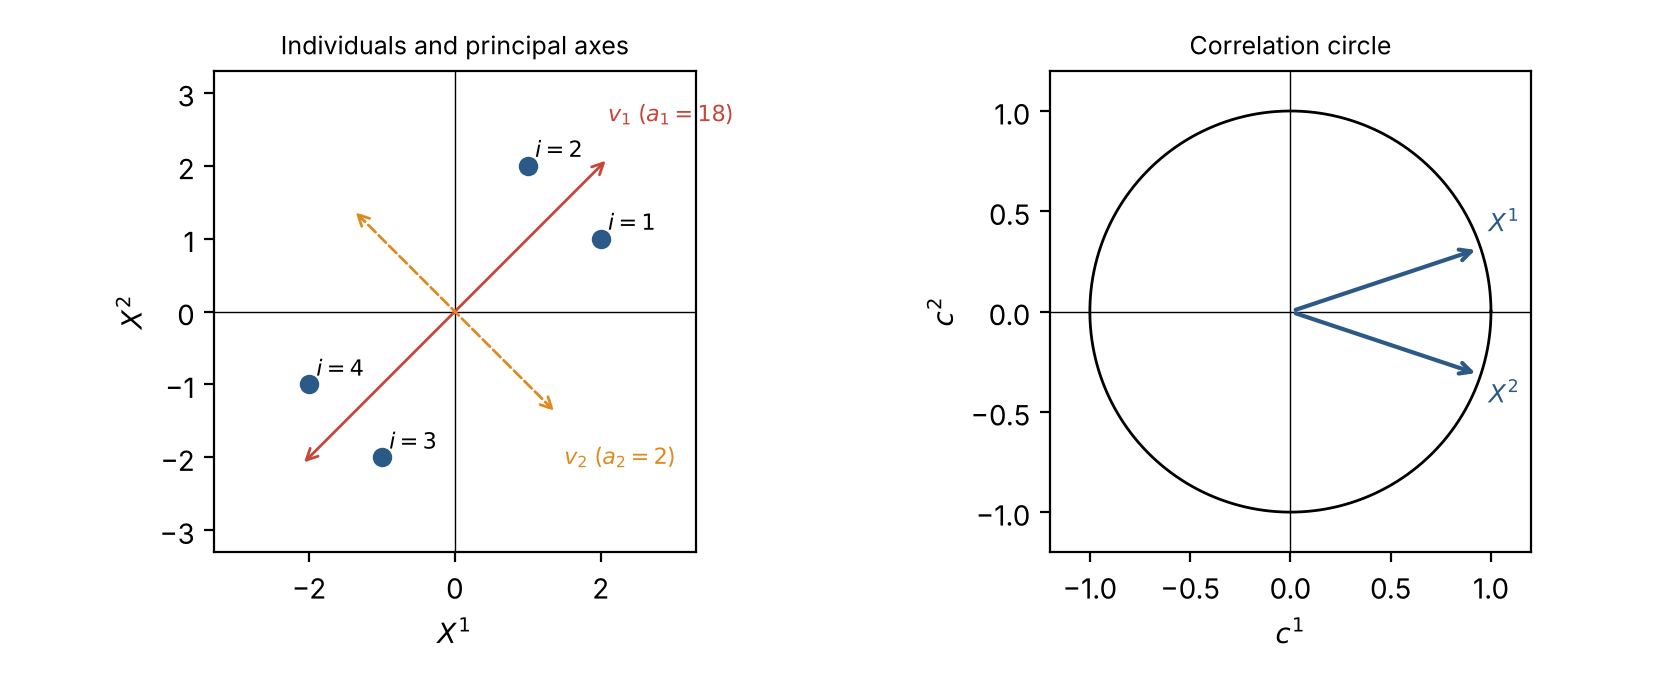
\includegraphics[width=0.88\textwidth]{pca_plots.png}\\[2pt]
{\footnotesize\textit{Left: individuals and principal axes $v_1, v_2$. Right: correlation circle, $X^1$ and $X^2$ are strongly correlated.}}
\end{center}

\vspace{4pt}
\begin{tcolorbox}[
    colframe=accentred,
    colback=white,
    arc=1.5mm,
    boxrule=0.5pt,
    left=8pt, right=8pt, top=5pt, bottom=5pt
]
\textbf{\color{accentred}Reading the circle.} Long arrows close to the circumference are well-represented by the retained axes; short arrows near the center are poorly represented and should not be interpreted.
\end{tcolorbox}

\end{document}
